\newpage
\section{Design Considerations}

% chktex-file 24
% chktex-file 8

\subsection{Data}
\label{subsec:design-data}

Table~\ref{tab:data} discusses the different types of data we are going to need to store and where they should be stored based upon their properties.


\begin{longtable}{ p{.12\textwidth} p{.1\textwidth} p{.1\textwidth} p{.63\textwidth} }
  \toprule
  \textbf{Data} & \textbf{Size} & \textbf{Location} & \textbf{Explanation}\\
  \midrule\midrule
  Game Metadata\newline\reqref{F-M1}
  & 100 -- \newline200B
  & Ethereum
  & This data is the minimal set of information required for the unique identification of each game. See Section~\ref{subsubsec:eth-data}.

  \vspace{1mm}
  This data is appropriate to store on Ethereum as it is public, small in size, and essential to the correct functioning of the application as all users will need to be able to discover all games. 
  \x
  Game Hash Tree\newline\reqref{F-M12}
  & \~15KB
  & IPFS
  & This will be the compressed Hash Tree that will allow the users to identify and verify the shards of data they need to download for their game. The user will download this immediately after purchasing the game.

  \vspace{1mm}
  This data would be costly to store on Ethereum for a large number of games and will only need to be accessed by a subset of users. As it is also public data, IPFS is appropriate to store it on, and we can reference the CID within the data stored on Ethereum.
  \x
  Game\newline Assets\newline\reqref{F-C2}
  & Unkown~\footnote{Some games may include many promotional materials, whilst some could include none. Therefore, it is hard to estimate the expected size.} 
  & IPFS
  & This will represent any promotional material provided for the game that can be viewed on the game's store page. This will typically include cover art and a markdown file for the description. The user will download this when they first view it in the store.

  \vspace{1mm}
  Similar to the Hash Tree, this will typically be too large to store on Ethereum so, given that it is public and non-essential data, IPFS will be used to store and distribute it. 
  \x
  Game Data
  & \textit{avg. 44GB~\footnote{Calculated based off of the top 30 games from SteamDB~\cite{noauthor_steam_nodate}.}}
  & Peers
  & This will the data required to play the game and will be fetched based upon the contents of the game's Hash Tree.

  \vspace{1mm}
  This data is way too large to store on Ethereum but also isn't public, which means using IPFS would not be appropriate~\footnote{IPFS and similar platforms provide no access control for the data stored there and any encryption based technique would be unviable.}. Therefore, this project will use a custom P2P network for sharing data, which is described in Section~\ref{subsec:design-p2p} 
  \\\bottomrule\bottomrule
  \caption{The different types of data required for each game.}
  \label{tab:data}
\end{longtable}

\noindent 
Swarm~\cite{hartman_swarm_1999} was considered as a decentralised storage and distribution platform over IPFS but was decided against as it would couple this project more tightly with Ethereum. On top of that, IPFS has much greater adoption and is much more mature in terms of working on a large scale.
\subsection*{Architecture}

Figure~\ref{fig:architecture-diagram} shows the architecture of this application:

\begin{figure}[ht]
  \centering
  \includegraphics*[width=\textwidth]{assets/images/diagrams/architecture-diagram.png}
  \caption{Architecture of the application}
  \label{fig:architecture-diagram}
\end{figure}

\subsection*{Sequence Diagram}

Figure~\ref{fig:sequence-diagram}, shows the main interactions between actors in the application.

\begin{figure}[ht]
  \centering
  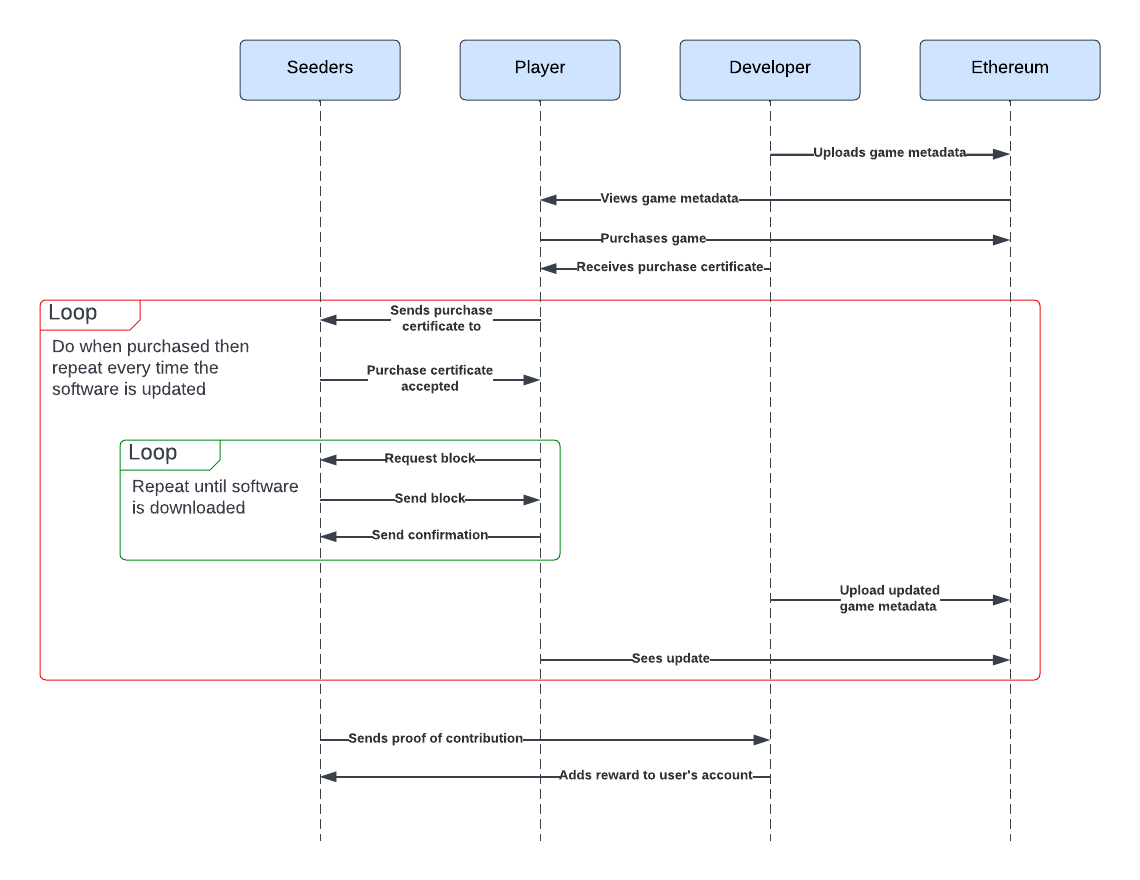
\includegraphics[width=.95\textwidth]{assets/images/diagrams/seqeunce-diagram.png}
  \caption{A sequence diagram showing some of the main interactions within this application}
  \label{fig:sequence-diagram}
\end{figure}



\subsection*{Blockchain}\label{subsec:design-con-eth}

\subsubsection*{Type of Blockchain}

To satisfy \reqref{NF-M1} and \reqref{NF-M2}, we will need to use a public blockchain. This will benefit my project by:
\vspace{2mm}
\begin{itemize}
  \item being accessible to more users, which will boost both availability and scalability \reqref{NF-S1},
  \item reducing the risk of censorship \reqref{NF-M1}, and
  \item providing greater data integrity \reqref{NF-M4}
\end{itemize}

\newparagraph Ethereum is a public blockchain that allows developers to publish their own distributed applications to it. It comes with an extensive development toolchain so is an obvious choice for this project \reqref{F-M4}.

\subsubsection*{Uploading Games}
\label{subsubsec:eth-data}



To satisfy \reqref{F-M1} and \reqref{F-M2}, the data stored on the blockchain will be used for the identification of games. Table~\ref{tab:eth-data} shows the fields that will stored as part of the smart contract for each game and to manage the whole collection of games. Fields in \textit{italics} are generated for the user and non-italic fields are entered manually.

\begin{longtable}{ p{.2\textwidth} p{.75\textwidth} }
  \toprule
  \textbf{Name} & \textbf{Description}
  \\\midrule\midrule
  \multicolumn{2}{c}{\textit{Metadata for each game}} 
  \\\midrule\midrule
  title & The name of the game.\\
  version & The version number of the game.\\
  \textit{release date} & The timestamp for when the game was uploaded.\\
  developer & The name of the developer uploading the game \reqref{NF-M3}.\\
  \textit{uploader} & The Ethereum address of the developer \reqref{NF-M3}.\\
  \textit{root hash} & The root hash of the game that uniquely identifies the game and is based upon its contents.\\
  previous version & The root hash of the most previous version of the game if it exists.\\
  price & The price of the game in Wei.\\
  \textit{hash tree CID} & Required for downloading the hash tree from IPFS.\\
  \textit{assets CID} & Required for downloading the assets folder from IPFS.
  \\\midrule\midrule
  \multicolumn{2}{c}{\textit{Managing the Collection of Games}} 
  \\\midrule\midrule
  \textit{library} & A mapping for all games uploaded to the network, where a game's root hash is the key used to find its metadata.\\
  \textit{game hashes} & Solidity doesn't allow us to enumerate maps so we will also store a list of hashes for all games uploaded.\\
  \textit{purchased} & A mapping which allows us to easily check if a user has purchased a game \reqref{F-M6}.
  \\\bottomrule\bottomrule
  \caption{the data to be stored on Ethereum using a smart contract}
  \label{tab:eth-data}
\end{longtable}


\subsubsection*{Purchasing Content}

Users will purchase games from developers over Ethereum by transferring Ether \reqref{F-M5}. The user's address will then be added to a public record, on the smart contract, of all users who have purchased the game \reqref{F-M6}. Upon purchasing a game, a user will broadcast their new library to all of their peers.

% chktex-file 1
% chktex-file 13

\subsection{Distributed File Sharing}
\label{subsec:design-p2p}

\subsubsection*{Hash Tree}
\label{subsubsec:hash-tree}

The hash tree of a given directory is used to represent its structure as well as the contents of its files. Each file is represented by an ordered list of SHA-256 hashes that match a fixed-size block of data. This allows users to easily identify and verify game data \reqref{F-M10}.

\begin{figure}[ht]
  \centering
  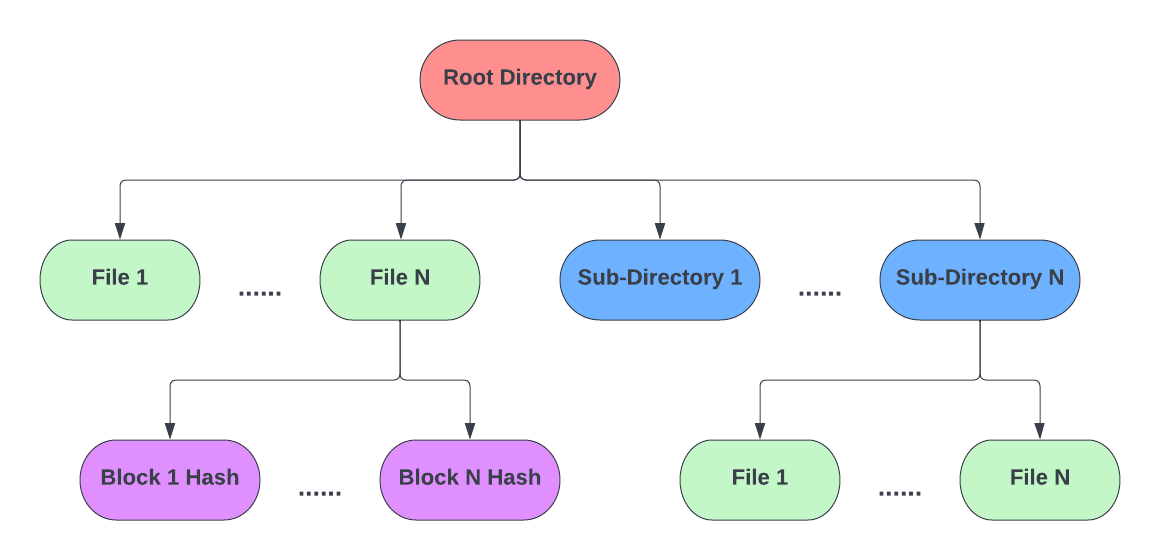
\includegraphics[width=.85\textwidth]{assets/images/diagrams/block-body.png}
  \caption{The structure of a hash tree}
  \label{fig:hash-storage}
\end{figure}

\subsubsection*{Uploading Content}
\label{subsubsec:upload-content}

For a developer to upload their game \reqref{F-M1}, they must provide the following:

\begin{itemize}
  \item the metadata outlined in Section~\ref{subsubsec:eth-data},
  \item a hash tree created from the root directory of the game, and
  \item an assets folder containing a piece of cover art \textit{(cover.png)} and a description file \textit{(description.md)}.
\end{itemize}

\vspace{2mm}\noindent
The developer should be able to enter the required fields into an upload page of the GUI and have the data generated and uploaded for them \reqref{F-S2}.

\subsubsection*{Downloading Content}

\newcommand{\seeder}{$P_{seeder}$~}
\newcommand{\downloader}{$P_{downloader}$~}

Like mentioned in Section~\ref{subsec:design-data}, it is impractical to store the game's data on the blockchain or IPFS. Instead we will consider ideas from decentralised file-sharing networks, like discussed in Sections~\ref{sec:lit-p2p} \&~\ref{sec:bittorrent}.
\x
Games are content addressable using their root hash field, which will allow users to request data from that game from other users. When a peer seeking data \downloader forms a connection with another peer \seeder they will:

\begin{enumerate}
  \item Perform a handshake to determine each other's Ethereum address and public key.
  \item \seeder will verify that \downloader owns the game by checking the \textit{purchased} mapping on the smart contract \reqref{F-M6} \reqref{F-S1}.
  \item \downloader will send requests for individual blocks to \seeder \reqref{F-M9}.
  \item Upon receiving a block, \downloader will verify the contents using the block's hash \reqref{F-M10} before writing it to disk in the appropriate location.
  \item Repeat Steps 3--4 until the entire game has been downloaded \reqref{F-M11}.
  \item \seeder may request a signed receipt that details the blocks they uploaded \reqref{F-S3} to \downloader.
\end{enumerate}

\vspace{2mm}\noindent
Users will be able to connect to many peers at once \reqref{F-M7} and will send download requests to the subset of their peers who also own the game. Requests will be sent in a round-robin fashion to evenly distribute the requests and prevent overloading a single peer \reqref{NF-S1}. Requests that cannot be completed will be retried when connecting to a new peer or when a peer has a change in library.

\subsubsection*{Updating Content}\label{subsubsec:updating}

To satisfy \reqref{F-M2}, developers will perform the same steps outlined in Section~\ref{subsubsec:upload-content} but must also provide the root hash of the most previous version of the game. Any users who have purchased the previous version will be added to the list of users who have purchased the new version \reqref{F-M3}. Additionally, this will include the restriction that only the original uploader can upload an update for their game \reqref{NF-M5}.
\x
Each version is considered its own game and will require users to download the updated version separately. Whilst this isn't reflective of how updates are typically managed, this will be acceptable for the scope of this project.

\subsubsection*{Downloadable Content}

Downloadable Content (DLC) \reqref{F-C1} represent optional additions for games that users will buy separately. DLCs will act similarly to how updates are treated. Each DLC will need:

\begin{enumerate}
  \item \textbf{Dependency} The root hash of the oldest version of the game this DLC supports.
  \item \textbf{Previous Version} (Optional) The root hash of the previous version of the DLC.
\end{enumerate}

\vspace{2mm}\noindent
Users must own the original game to buy any of its DLC. 

\subsubsection*{Proving Contribution}

As a user downloads blocks of data, they will keep track of which users have sent them which blocks. A peer may then request their contributions in the form of a signed message that can be sent to the developer \reqref{F-S3} in return for some kind of reward. The contents of the reward isn't specified for this project but could include in-game items, digital assets or Ether. This solution assumes that developers have knowledge of which Ethereum address maps to which of their game's users.

\subsection*{Downloading Content}

Games will be content addressable, using their root hash stored on the blockchain. This will be used to help connect nodes who are interested in the same content (\textbf{F\_M3}). Once a user connects to a node it will:
\vspace{2mm}
\begin{enumerate}
  \item Send their proof of purchase (\textbf{F\_S2}).
  \item request individual shards from the node using the shard's hash (\textbf{F\_M2}),
  \item use the metadata from the blockchain to verify the shard's contents (\textbf{F\_M7}),
  \item send a confirmation message that proves the successful transfer of a block (\textbf{F\_S1}),
  \item and repeat this until the entirety of the game is installed (\textbf{F\_M6}).
\end{enumerate}

\vspace{2mm}\noindent As the blockchain will only be used to store metadata about games uploaded to the network, not every node will have each game installed. Instead, this project will take ideas from networks like BitTorrent, where nodes will seek out peers who have the game installed using a tracker hosted by the uploader.

\subsection*{Updating Content}

To satisfy \textbf{F\_M4}, developers will perform the same steps as in \textbf{Uploading Content} but will also include the hash of a previous block that contains the older version of the game. This relationship will allow users ownership to all versions of a game they have purchased and not just a singular version. This will include the restriction that only the original uploader can upload an update for their game (\textbf{NF\_S2}).

\vspace{2mm}\noindent Each version will be considered as a standalone game and will require users to download the entirety by scratch. Whilst this isn't reflective of how updates are typically managed, this will be acceptable for the scope of this project and any changes will be considered as a future extension to this project.

\subsubsection*{Downloadable Content}

Developers will typically offer paid or free DLC (\textbf{F\_S3}) for their games that users will purchase separately. Each DLC will need:

\begin{enumerate}
  \item \textbf{Dependency} A reference to the oldest version of the game they apply to, and
  \item \textbf{Previous Version} A pointer to the previous version of the DLC.
\end{enumerate}

\begin{figure}[ht]
  \centering
  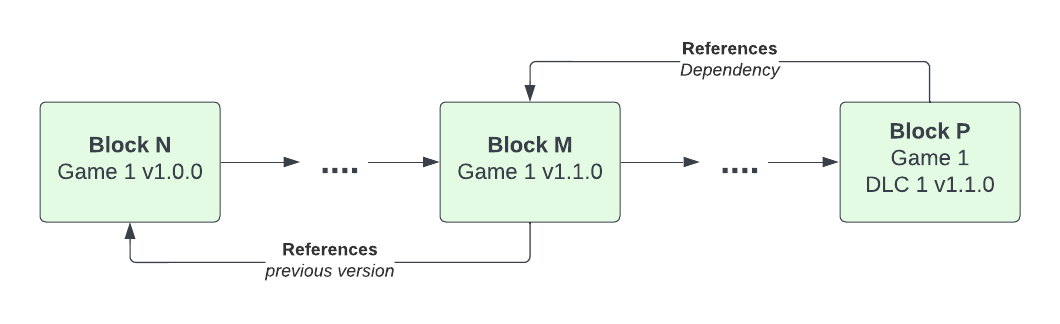
\includegraphics[width=.85\textwidth]{assets/images/diagrams/software.png}
  \caption{How blocks relate to each other. An update will reference the previous version whilst a DLC will reference, which piece of software and version it is dependent on.}
\end{figure}

\subsection*{Proving Contribution}

A purchase certificate will include a confidential \textit{seeder token}. When a user successful downloads a shard of data they will send a confirmation message, including their seeder token, that is encrypted with the game developer's public key. A user will prove their contribution (\textbf{F\_S1}) by sending a collection of these messages to the developer, who can decrypt and validate the tokens.
